% Escena POMDP sobre la rejilla. \ejeH y \ejeV dan el nombre de los ejes (c/r o x/y).
\providecommand{\ejeH}{c}
\providecommand{\ejeV}{r}
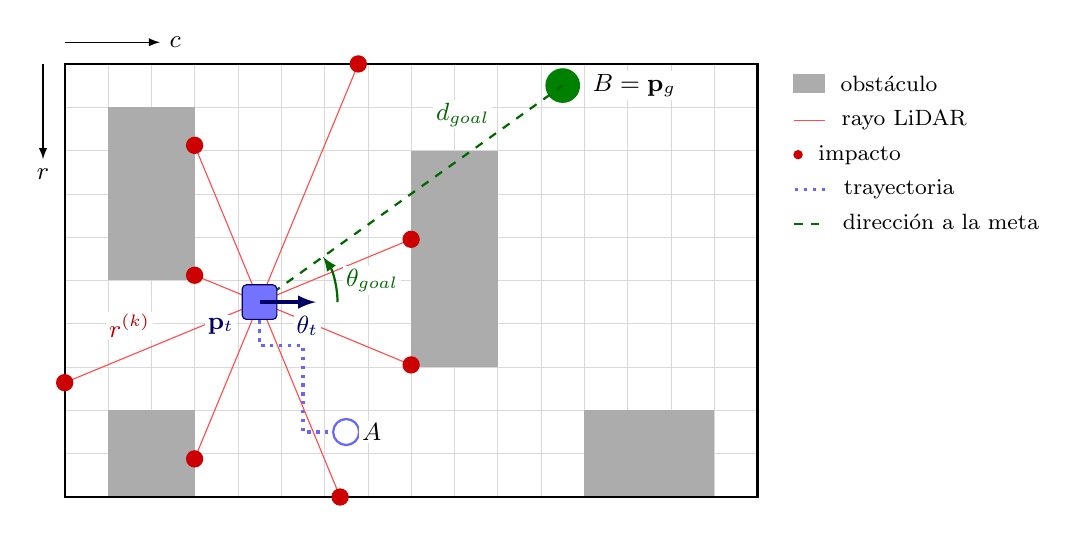
\begin{tikzpicture}[scale=0.55, >=latex,
        etiq/.style={fill=white, inner sep=1pt, font=\small}]
    \draw[gray!30, very thin] (0,0) grid (16,10);
    \fill[gray!65] (8,3) rectangle (10,8);
    \fill[gray!65] (1,5) rectangle (3,9);
    \fill[gray!65] (1,0) rectangle (3,2);
    \fill[gray!65] (12,0) rectangle (15,2);
    \draw[thick] (0,0) rectangle (16,10);
    \draw[->] (0,10.5) -- (2.2,10.5) node[right] {\small $\ejeH$};
    \draw[->] (-0.5,10) -- (-0.5,7.8) node[below] {\small $\ejeV$};
    % Trayectoria recorrida desde el punto de partida A
    \draw[blue!60, dotted, very thick]
        (6.5,1.5) -- (5.5,1.5) -- (5.5,3.5) -- (4.5,3.5) -- (4.5,4.5);
    % Rayos del LiDAR (uno por sector) hasta el primer impacto
    \foreach \p in {(8,5.95), (6.78,10), (3,8.12), (3,5.12),
                    (0,2.64), (3,0.88), (6.36,0), (8,3.05)} {
        \draw[red!70, thin] (4.5,4.5) -- \p;
        \fill[red!80!black] \p circle (0.2);
    }
    \node[etiq, text=red!70!black] at (1.5,3.95) {$r^{(k)}$};
    \fill[white, draw=blue!60, thick] (6.5,1.5) circle (0.3);
    \node[etiq, right=3pt] at (6.6,1.5) {$A$};
    % Meta B, distancia y rumbo a la meta
    \fill[green!50!black] (11.5,9.5) circle (0.4);
    \node[etiq, right=8pt] at (11.6,9.5) {$B = \mathbf{p}_g$};
    \draw[green!40!black, dashed, thick] (4.5,4.5) -- (11.5,9.5)
        node[etiq, pos=0.78, above left=1pt, text=green!40!black]
        {$d_{\text{goal}}$};
    \draw[->, green!40!black, thick] (6.3,4.5) arc (0:35.5:1.8);
    \node[etiq, text=green!40!black] at (7.1,5.0) {$\theta_{\text{goal}}$};
    % AGV con su orientación
    \draw[fill=blue!55, draw=blue!40!black, rounded corners=1.5pt]
        (4.1,4.1) rectangle (4.9,4.9);
    \draw[->, very thick, blue!40!black] (4.5,4.5) -- (5.8,4.5);
    \node[etiq, text=blue!40!black] at (5.6,3.95) {$\theta_t$};
    \node[etiq, text=blue!40!black] at (3.6,3.95) {$\mathbf{p}_t$};
    % Leyenda
    \node[anchor=north west, align=left, font=\footnotesize] at (16.6,10) {
        \tikz[baseline=-0.6ex]\fill[gray!65] (0,-0.1) rectangle (0.4,0.15);
            \ obstáculo\\[3pt]
        \tikz[baseline=-0.6ex]\draw[red!70] (0,0) -- (0.4,0);
            \ rayo LiDAR\\[3pt]
        \tikz[baseline=-0.6ex]\fill[red!80!black] (0.2,0) circle (0.06);
            \ impacto\\[3pt]
        \tikz[baseline=-0.6ex]\draw[blue!60, dotted, very thick] (0,0) -- (0.4,0);
            \ trayectoria\\[3pt]
        \tikz[baseline=-0.6ex]\draw[green!40!black, dashed, thick] (0,0) -- (0.4,0);
            \ dirección a la meta
    };
\end{tikzpicture}
